\documentclass[preprint, 3p,
authoryear]{elsarticle} %review=doublespace preprint=single 5p=2 column
%%% Begin My package additions %%%%%%%%%%%%%%%%%%%

\usepackage[hyphens]{url}

  \journal{An awesome journal} % Sets Journal name

\usepackage{graphicx}
%%%%%%%%%%%%%%%% end my additions to header

\usepackage[T1]{fontenc}
\usepackage{lmodern}
\usepackage{amssymb,amsmath}
% TODO: Currently lineno needs to be loaded after amsmath because of conflict
% https://github.com/latex-lineno/lineno/issues/5
\usepackage{lineno} % add
\usepackage{ifxetex,ifluatex}
\usepackage{fixltx2e} % provides \textsubscript
% use upquote if available, for straight quotes in verbatim environments
\IfFileExists{upquote.sty}{\usepackage{upquote}}{}
\ifnum 0\ifxetex 1\fi\ifluatex 1\fi=0 % if pdftex
  \usepackage[utf8]{inputenc}
\else % if luatex or xelatex
  \usepackage{fontspec}
  \ifxetex
    \usepackage{xltxtra,xunicode}
  \fi
  \defaultfontfeatures{Mapping=tex-text,Scale=MatchLowercase}
  \newcommand{\euro}{€}
\fi
% use microtype if available
\IfFileExists{microtype.sty}{\usepackage{microtype}}{}

\ifxetex
  \usepackage[setpagesize=false, % page size defined by xetex
              unicode=false, % unicode breaks when used with xetex
              xetex]{hyperref}
\else
  \usepackage[unicode=true]{hyperref}
\fi
\hypersetup{breaklinks=true,
            bookmarks=true,
            pdfauthor={},
            pdftitle={Aplicativo interativo de mineração de textos para análises de experiências turísticas},
            colorlinks=false,
            urlcolor=blue,
            linkcolor=magenta,
            pdfborder={0 0 0}}

\setcounter{secnumdepth}{5}
% Pandoc toggle for numbering sections (defaults to be off)


% tightlist command for lists without linebreak
\providecommand{\tightlist}{%
  \setlength{\itemsep}{0pt}\setlength{\parskip}{0pt}}


% Pandoc citation processing
\newlength{\cslhangindent}
\setlength{\cslhangindent}{1.5em}
\newlength{\csllabelwidth}
\setlength{\csllabelwidth}{3em}
\newlength{\cslentryspacingunit} % times entry-spacing
\setlength{\cslentryspacingunit}{\parskip}
% for Pandoc 2.8 to 2.10.1
\newenvironment{cslreferences}%
  {}%
  {\par}
% For Pandoc 2.11+
\newenvironment{CSLReferences}[2] % #1 hanging-ident, #2 entry spacing
 {% don't indent paragraphs
  \setlength{\parindent}{0pt}
  % turn on hanging indent if param 1 is 1
  \ifodd #1
  \let\oldpar\par
  \def\par{\hangindent=\cslhangindent\oldpar}
  \fi
  % set entry spacing
  \setlength{\parskip}{#2\cslentryspacingunit}
 }%
 {}
\usepackage{calc}
\newcommand{\CSLBlock}[1]{#1\hfill\break}
\newcommand{\CSLLeftMargin}[1]{\parbox[t]{\csllabelwidth}{#1}}
\newcommand{\CSLRightInline}[1]{\parbox[t]{\linewidth - \csllabelwidth}{#1}\break}
\newcommand{\CSLIndent}[1]{\hspace{\cslhangindent}#1}

\usepackage{hyperref}
\hypersetup{ colorlinks=true, linkcolor=black, urlcolor=green }
\urlstyle{same}
\usepackage{booktabs}
\usepackage{longtable}
\usepackage{array}
\usepackage{multirow}
\usepackage{wrapfig}
\usepackage{float}
\usepackage{colortbl}
\usepackage{pdflscape}
\usepackage{tabu}
\usepackage{threeparttable}
\usepackage{threeparttablex}
\usepackage[normalem]{ulem}
\usepackage{makecell}
\usepackage{xcolor}



\begin{document}


\begin{frontmatter}

  \title{Aplicativo interativo de mineração de textos para análises de
experiências turísticas}
    \author[Some Institute of Technology]{Author1%
  \corref{cor1}%
  \fnref{1}}
   \ead{a@example.com} 
    \author[Another University]{Author2%
  %
  }
   \ead{b@example.com} 
    \author[Another University]{Author3%
  %
  \fnref{2}}
   \ead{c@example.com} 
      \affiliation[Some Institute of Technology]{Department, Street,
City, State, Zip}
    \affiliation[Another University]{Department, Street, City, State,
Zip}
    \cortext[cor1]{Corresponding author}
    \fntext[1]{This is the first author footnote.}
    \fntext[2]{Another author footnote.}
  
  \begin{abstract}
  Investigating the experience economy, observing the levels of
  interaction experienced by tourists in destinations, can be an
  important tool for the best use of and sustainable development of
  tourist regions. This article presents an approach for evaluating the
  domains of experience of tourist attractions based on comments posted
  on the Tripadvisor platform. The interpretation was performed using
  netnography, through text mining techniques, natural language
  processing and text classification with machine learning. The
  attractions were evaluated and classified considering the reported
  experiences. The approach presented here contributes to the
  identification of gaps regarding public and private initiatives that
  make it possible to meet the expectations of tourists, making the most
  competitive and viable tourist spots in terms of sustainable
  development. The methodological conception of the research can
  constitute an important tool for the study of tourism and enable
  theoretical deepening and improvements in the offer of ecotourism
  products.
  \end{abstract}
    \begin{keyword}
    Experience Economics \sep Text Mining \sep Natural Language
Processing \sep Machine Learning \sep 
    Textual Analysis Tool
  \end{keyword}
  
 \end{frontmatter}

\hypertarget{resumo}{%
\section{Resumo}\label{resumo}}

Investigar a economia da experiência, observando os níveis de interação
vivenciados pelos turistas, pode ser uma importante ferramenta para o
melhor aproveitamento e desenvolvimento sustentável de regiões
turísticas. Este artigo apresenta uma abordagem para a avaliação dos
domínios da experiência de pontos turísticos a partir dos comentários
postados na plataforma \emph{Tripadvisor}. Foi construído um aplicativo
interativo e amigável para auxiliar na interpretação e classificação das
experiências relatadas pelos turistas, empregando-se a netnografia,
através de técnicas de mineração de textos, processamento de linguagem
natural e classificação de textos com aprendizado de máquina. A
abordagem aqui apresentada contribui para a identificação de lacunas no
que tange iniciativas públicas e privadas que possibilitem o atendimento
das expectativas dos turistas, tornando os pontos turísticos mais
competitivos e viáveis na perspectiva do desenvolvimento sustentável. A
concepção metodológica da pesquisa pode se constituir em uma importante
ferramenta para o estudo do turismo e possibilitar aprofundamentos
teóricos e melhorias da oferta de produtos do ecoturismo.

\emph{palavras-chave}: Economia da Experiência, Mineração de Textos,
Processamento de Linguagem Natural, Aprendizado de Máquina, Ferramentas
de Análise textual

\hypertarget{introduuxe7uxe3o}{%
\section{Introdução}\label{introduuxe7uxe3o}}

O turismo constitui-se em um complexo processo de decisão realizado por
diferentes motivações como, por exemplo, a hospedagem, a alimentação, o
lazer, a informação turística, o entretenimento, dentre outras variáveis
(\protect\hyperlink{ref-beni2019}{M. C. Beni 2019}). Os serviços
turísticos não podem ser entendidos como um produto estático, pois eles
necessitam de evolução para o crescimento do turismo no Brasil e no
mundo (\protect\hyperlink{ref-Coelho2007}{Coelho and Ribeiro 2007}). Tal
avanço também perpassa pelo consumidor, visto que ele busca, muito além
de produtos e serviços turísticos, novas experiências, alterando gostos
e preferências referentes à demanda anterior
(\protect\hyperlink{ref-Beni2004}{Mário Carlos Beni 2004}).

Segundo (\protect\hyperlink{ref-Beni2004}{Mário Carlos Beni 2004})
deve-se buscar a harmonia entre o que o destino turístico pode oferecer
e as experiências turísticas que o visitante busca ao viajar. Há uma
mudança significativa nos gostos e preferências dos turistas, que
anteriormente buscavam produtos e serviços, e atualmente a procura
perpassa, também, pela ambição de experiências novas
(\protect\hyperlink{ref-Beni2004}{Mário Carlos Beni 2004}). Essas
experiências, entendidas como uma avaliação que o sujeito faz de forma
subjetiva quando há submissão às experimentações turísticas (afetivas,
cognitivas e comportamentais) se iniciam com a preparação para a
imersão, se alongam durante ela, e estendem-se até a completude da
experiência, deixando bastante evidente a amplitude de significados
gerados pelas experiências (\protect\hyperlink{ref-Tung2011}{Tung and
Ritchie 2011}). Dessa forma, o resultado torna-se extenso, passando pela
fidelização do consumidor, a perpetuação do sentido experienciado em sua
memória e até a recomendação para outros potenciais consumidores
(\protect\hyperlink{ref-Coelho2007}{Coelho and Ribeiro 2007};
\protect\hyperlink{ref-Alencar2019}{Alencar et al. 2019};
\protect\hyperlink{ref-LoBuono2016}{LoBuono et al. 2016}).

Diante dessa perspectiva, Pine and Gilmore
(\protect\hyperlink{ref-pine1999}{1998}) fazem uma diferenciação quanto
aos serviços e as experiências: respectivamente, de um lado tem-se um
conjunto de atividades intangíveis, e do outro, eventos ou experiências
memoráveis. Estas experiências memoráveis são planejadas para engajar o
turista ao processo, e não somente entretê-lo. Assim, quatro domínios de
experiência foram propostos, a partir de dois eixos, chamados de
estágios da estruturação de uma experiência (Figura \ref{fig:figura1}).

\begin{figure}[H]
  \centering
  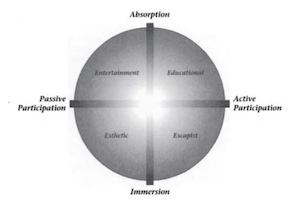
\includegraphics[width=0.5\textwidth]{./fig1.jpeg}
  \caption{Categorias utilizadas para a classificação da experiência Fonte: Pine e Gilmore (1999)}
  \label{fig:figura1}
\end{figure}

O primeiro dos eixos, proposto horizontalmente, refere-se à participação
do indivíduo, podendo ser classificada como passiva (passive
participation) ou ativa (active participation). Já o eixo vertical
representa o aspecto ambiental que interliga indivíduo e experiência: de
um lado está a imersão (immersion) e do outro a absorção (absorption). O
cruzamento desses dois eixos cria as quatro dimensões ou domínios de
experiência: entretenimento, aprendizagem, estética e evasão/escapismo
(\protect\hyperlink{ref-pine1999}{Pine and Gilmore 1998}).

O primeiro quadrante envolve a dimensão caracterizada como
\textbf{entretenimento}. É quando o turista busca experiências que sejam
divertidas e emocionantes, como parques de diversão, shows, esportes
radicais, vida noturna ou atividades em grupo. Trata-se de uma dimensão
mais passiva, em que o indivíduo responde aos elementos que lhe são
apresentados levando-o a expressar sinais de satisfação, riso e
relaxamento. Dessa forma, a fim de desenvolver um serviço turístico que
contemple esta dimensão, deve-se torná-lo mais divertido e admirado
(\protect\hyperlink{ref-Horodyski2015}{Horodyski, Fernandes, and Gândara
2015}; \protect\hyperlink{ref-Alencar2019}{Alencar et al. 2019};
\protect\hyperlink{ref-Hott2023}{Corrêa and Gosling 2023}). Em vista
disso pode-se resumir que se trata de oferecer opções pessoais de lazer
no destino escolhido.

A segunda dimensão consiste na \textbf{aprendizagem}. Envolve uma
participação ativa do indivíduo com a atividade turística. É quando o
turista busca uma experiência que o faça aprender algo novo, como uma
cultura diferente, um idioma, uma habilidade ou conhecimento histórico.
O aprender demanda que o sujeito interaja e se envolva com o objeto de
apreensão. Nesse sentido, ao se preparar um serviço que contemple a
economia da experiência, deve-se definir quais informações pretende-se
que o turista absorva, como também, quais habilidades pretende-se que o
mesmo pratique durante o consumo, implicando em vivenciar tanto a
perspectiva sensorial quanto intelectual LoBuono et al.
(\protect\hyperlink{ref-LoBuono2016}{2016}). Aqui depreende-se que
contemple a obtenção de contato com aspectos do ambiente, da cultura e
da história dos habitantes do local/região visitado.

A terceira dimensão corresponde à \textbf{estética/contemplação}. É
quando o turista busca experiências que envolvam a apreciação da beleza,
seja ela natural ou criada pelo homem. Isso pode incluir visitas a
museus, galerias de arte, parques naturais ou cidades históricas. Essa
dimensão abrange elementos que atraem o indivíduo por razões visuais,
fazendo com que tome a decisão de adentrar em um local e ali permanecer.
Cabe ressaltar que a escolha em incluir a ``contemplação'' no conceito
original Pine and Gilmore (\protect\hyperlink{ref-pine1999}{1998}) parte
do estudo de Andrukiu and Gândara
(\protect\hyperlink{ref-Andrukiu2015}{2015}) que considera a dimensão da
contemplação como um fator característico da ``estética''. Ao se propor
a oferta de um serviço, a fim de que proporcione ao turista vivenciar
esta dimensão, deve-se criar um ambiente convidativo, interessante e
confortável, para que ele se sinta impelido a ficar ali. Pode-se inferir
que esta dimensão se caracteriza com a qualidade aparente dos atrativos
visitados, que despertam no indivíduo a conduta de admirar o ambiente.

A quarta dimensão refere-se a \textbf{evasão/escapismo}. É quando o
turista busca uma experiência que o ajude a escapar da realidade e do
estresse do dia a dia. Isso pode incluir viagens para lugares isolados e
tranquilos, retiros espirituais, spas, praias ou montanhas. Diz respeito
à capacidade de fazer com que o turista fique imerso nas atividades que
lhe são propostas. Ao desenvolver produtos turísticos, deve-se criar
condições que possibilitem ao indivíduo vivenciar situações que lhe
demandem uma participação ativa, bem como, despertem nele (o domínio dos
seus sentidos), uma completa imersão, suscitando a manifestação de
sentimentos e emoções. Pode-se dizer que esta dimensão implica em
sensações de desprendimento pessoal. Já Aroeira, Dantas, and Gosling
(\protect\hyperlink{ref-Aroeira2016}{2016}), classifica experiências
dessa natureza como equivalentes ao pensamento, à absorção e imaginação
do cliente, como por exemplo, o ``desligar'', ``se conectar'' com o
lugar.

É importante lembrar que esses domínios não são mutuamente exclusivos e
que muitas vezes uma única experiência pode incluir elementos de mais de
um domínio. Além disso, a maneira como os turistas experimentam cada um
desses domínios pode variar de acordo com suas personalidades,
interesses e expectativas. Dessa forma, para que a experiência seja
memorável, deve-se proporcionar ao turista vivenciar as quatro
dimensões. Essa perspectiva analítica oferece ao produtor de serviço
turístico, um diagnóstico que permite compreender o atendimento da
expectativa do cliente, nestas quatro dimensões, exibindo opções e
diretrizes que possam proporcionar uma melhor experiência ao mesmo.

\hypertarget{apresentauxe7uxe3o-da-abordagem-realizada}{%
\subsection{Apresentação da abordagem
realizada}\label{apresentauxe7uxe3o-da-abordagem-realizada}}

Muitas pessoas e empresas utilizam a internet diariamente para expressar
suas opiniões, aumentando a quantidade de dados textuais existente, como
é o caso da plataforma \emph{TripAdvisor}. Esses dados podem conter
informações valiosas, que muitas vezes, podem ser obtidas com rapidez e
baixo custo financeiro, através de técnicas de mineração de texto e
processamento de linguagem natural (PLN), as quais envolvem o uso de
tecnologias computacionais para processar e analisar dados em linguagem
natural (\protect\hyperlink{ref-medeiros2021}{Tereza Medeiros 2021}).

A mineração de textos envolve a extração de informações úteis e
conhecimento a partir de grandes volumes de texto não estruturado, como
documentos, artigos, posts de redes sociais, entre outros. O objetivo é
transformar esse texto em dados estruturados, tornando-o mais fácil de
ser analisado. As principais etapas da mineração de textos incluem:
pré-processamento (limpeza, tokenização, stemming), análise de
sentimentos, extração de informações (entidades, relações),
classificação e clusterização (\protect\hyperlink{ref-Sharma2020}{Sharma
and Rana 2020}; \protect\hyperlink{ref-Yadav2018}{Yadav, Chahande, and
Wandre 2018}).

Já o processamento da linguagem natural é uma área da inteligência
artificial que envolve a compreensão da linguagem humana e a geração de
respostas adequadas em linguagem natural, normalmente envolvendo
algoritmos de aprendizagem de máquina, que podem ser supervisionados,
quando os dados já classificados efetivamente definem as categorias e
são usados como ``dados de treinamento'' para construir modelos que
possam ser usados para classificar novos dados
(\protect\hyperlink{ref-Tan1999}{Tan 1999}); ou não supervisionados,
quando não existem categorias pré-definidas. Uma das técnicas PNL não
supervisionada é a análise de tópicos, que permite identificar os
principais temas e conceitos presentes em um conjunto de dados textuais,
como avaliações de usuários e comentários em redes sociais, permitindo
identificar padrões e tendências nos comportamentos dos turistas, bem
como as percepções e opiniões dos viajantes sobre destinos, atrações e
serviços turísticos (\protect\hyperlink{ref-Silge2017}{Silge and
Robinson 2017}).

Uma questão central na mineração de textos e no processamento de
linguagem natural é como quantificar do que se trata um documento. Uma
medida de quão importante uma palavra pode ser é sua frequência de termo
(\texttt{tf}), ou seja, a frequência com que uma palavra ocorre em um
documento. Outra abordagem é observar a frequência inversa de documento
(\texttt{idf}) de um termo, que diminui o peso das palavras comumente
usadas e aumenta o peso das palavras que não são muito usadas em uma
coleção de documentos. Isso pode ser combinado com a frequência do termo
para calcular o \texttt{tf-idf} de um termo (as duas quantidades
multiplicadas juntas), ou seja, a frequência de um termo ajustada para
quão raramente ele é usado (\protect\hyperlink{ref-Fay2018}{Fay 2018}).

Zipf (1949) mostrou que uma das características das linguagens humanas,
populações das cidades e muitos outros fenômenos humanos e naturais,
seguem uma distribuição similar, a qual denominou de ``Princípio do
Menor Esforço''. Esta lei de Zipf define que, tomando um determinado
texto, o produto \(k_{t}\log(f_{t})\) é aproximadamente constante, em
que \(f_{t}\) é o número de vezes que o termo \(_t\) ocorre no texto e
\(k_{t}\) é a posição deste termo em uma relação de todos os termos
daquele texto, ordenados pela frequência de ocorrência
(\protect\hyperlink{ref-Bakulina2008}{Bakulina 2008}).

Por outro lado, Luhn sugeriu, em 1958, que a frequência de ocorrência
das palavras em um texto pode fornecer uma medida útil sobre a
expressividade das mesmas, pois o ``autor normalmente repete
determinadas palavras ao desenvolver ou variar seus argumentos e ao
elaborar diferentes enfoques sobre do que se trata o assunto''. As
palavras com maior frequência de ocorrência deveriam ser consideradas
pouco expressivas porque este conjunto de palavras é composto
normalmente por artigos, preposições e conjunções. Também as palavras
que muito raramente ocorrem deveriam ser consideradas pouco expressivas
justamente em razão da baixa frequência. Restam como expressivas as
palavras com maior frequência de ocorrência intermediária
(\protect\hyperlink{ref-Bezerra2014}{Bezerra and Guimarães 2014}).

Dessa forma, medidas de frequência de termos são valiosas nas análises
textuais. Esses termos são definidos como \emph{tokens}, ou seja, uma
unidade significativa de texto, que podem ser palavras, uma sequência
delas, frases, parágrafos, entre outros. Portanto, a tokenização é uma
etapa importante do processamento de linguagem natural e é usada em
muitas aplicações, como a classificação de textos. Os n-gramas, por sua
vez, são conjuntos de n tokens adjacentes em um texto
(\protect\hyperlink{ref-Silge2017}{Silge and Robinson 2017}). A escolha
do melhor método de tokenização e do tamanho dos n-gramas depende do
objetivo do problema. O tamanho ideal dos n-gramas depende do tamanho do
texto e da complexidade do problema. N-gramas maiores podem ajudar a
capturar contextos mais amplos, mas podem levar a um aumento na
dimensionalidade e na esparsidade dos dados, o que pode prejudicar o
desempenho de modelos. O tamanho ideal dos n-gramas é geralmente
determinado empiricamente, testando-se vários valores em um conjunto de
dados de validação (\protect\hyperlink{ref-Hvitfeldt2021}{Hvitfeldt and
Silge 2021}).

Nesse contexto, esta pesquisa tem como objetivo disponibilizar uma
ferramenta informatizada que possa ser utilizada para a análise dos
níveis de experiência e de satisfação de turistas em ambientes naturais,
empregando-se técnicas de mineraçao de textos e processamento de
linguagem natural. A partir das análises geradas, será possível definir
quais os n-gramas mais adequados para serem rotulados com as categorias
entretenimento, aprendizagem, estética e escapismo, possibilitando a
utilização de algoritmos de aprendizado supervisionado para a
classificação dos textos. Assim, modelos de \emph{machine learning}
poderão ser treinados para classificar os comentários em cada uma das
categorias, através de algoritmos como regressão logística, árvores de
decisão e redes neurais. Estudos de casos de pontos turísticos da
plataforma \emph{Tripadvisor} serão apresentados neste artigo, de forma
ilustrativa para evidenciar e validar a ferramenta desenvolvida.
Portanto, pretende-se com o trabalho, gerar um instrumento que possa ser
generalizado e utilizado para qualquer ponto turístico.

\hypertarget{material-e-muxe9todos}{%
\section{Material e Métodos}\label{material-e-muxe9todos}}

Foi construído um aplicativo usando o pacote \emph{Shiny} do ambiente R
de computação estatística, com a proposta de fornecer informações
suficientes para contribuir na análise de experiências turísticas. Foi
utilizado o \emph{software} estatístico R, que incorpora as
características de software livre, e o \emph{Rstudio}, que é o ambiente
de desenvolvimento integrado (IDE) para a linguagem R. O aplicativo foi
desenvolvido utilizando o \emph{Shiny}, framework que possibilita a
criação de aplicações interativas na web, não sendo necessário ao
programador ter conhecimento de HTML, CSS ou Javascript. Ele possui um
conjunto de funções destinadas a promover a interface com o usuário
(\emph{ui}), onde são coletadas informações fornecidas pelo mesmo, e
enviadas para o \emph{server}, cujo papel é processar as informações
coletadas e retorná-las para ui, que dará o \emph{feedback} ao usuário
(\protect\hyperlink{ref-Xie2016}{Xie 2016};
\protect\hyperlink{ref-RStudio2018}{RStudio 2018};
\protect\hyperlink{ref-Johnson2020}{Johnson 2020}).

Para realizar a análise da experiência turística de acordo com os quatro
domínios da experiência, foram selecionados dois pontos turísticos da
Plataforma \emph{TripAdvisor}:
\href{https://www.tripadvisor.com.br/Attraction_Review-g668997-d17816411-Reviews-JALAPAO_OFICIAL-Palmas_State_of_Tocantins.html}{Jalapão}
e
\href{https://www.tripadvisor.com.br/Tourism-g3842996-Ilha_do_Superagui_State_of_Parana-Vacations.html}{Superagui}.
A aquisição dos dados consistiu em obter os comentários dos turistas da
plataforma \emph{TripAdvisor}, utilizando técnicas de captura de dados
(\emph{web scraping})
(\protect\hyperlink{ref-munzert2014automated}{Munzert et al. 2014}) para
a extração automatizada dos dados, através do pacote \emph{rvest}
(\protect\hyperlink{ref-Wickham2019}{Wickham 2019}) do \emph{software}
R. Também foi utilizada a função \emph{gsub} para retirar as marcações
do \emph{html} e obter o texto sem formatação.

Após a importação dos dados, e antes de realizar as análises, foi
realizado um \textbf{pré-processamento} do mesmos. Este envolveu a
transformação das palavras em letras minúsculas, retirada de pontuação e
caracteres especiais (p.ex. ``!'', ``@'', ``\#'',``\$'') e eliminação de
espaços em branco. Existem algumas funções disponíveis para remoção da
pontuação, porém algumas substituem a pontuação por espaços e outras
não. A função \texttt{removePunctuation} do pacote \emph{tm} é muito
utilizada, mas deve ser utilizada com cuidado. O ideal é que sua
utilização seja somente em arquivos no formato \emph{corpus} em que as
palavras já estão separadas. Atenção também deve ser dada aos caracteres
especiais, por exemplo o @, pois estes também podem ou não ser
substituídos por espaço, alterando o resultado das análises
(\protect\hyperlink{ref-Hocking2019}{Hocking 2019}).

Em geral as expressões regulares são uma ferramenta poderosa e flexível
para trabalhar com texto e foram utilizadas nesse estudo. Elas são
amplamente utilizadas em programação e em sistemas de busca e análise de
dados, e podem ajudar a automatizar tarefas que envolvem manipulação de
texto. As expressões regulares permitem que você especifique um conjunto
de caracteres ou um padrão de caracteres que correspondem a uma
determinada sequência de texto, para realizar operações de substituição
e validação de texto (\protect\hyperlink{ref-RStudio2017}{RStudio
2017}).

Como parte do processo de limpeza ou pré-processamento do texto está a
remoção de caracteres repetidos. A função
\texttt{gsub("(\textbackslash{}\textbackslash{}w)\textbackslash{}\textbackslash{}1+",\ "\textbackslash{}\textbackslash{}1",\ data,\ perl\ =\ TRUE)}
utiliza expressões regulares para manipulação de strings. A expressão
regular
\texttt{(\textbackslash{}\textbackslash{}w)\textbackslash{}\textbackslash{}1+}
busca por qualquer caractere alfanumérico
\texttt{(\textbackslash{}\textbackslash{}w)} seguido por uma ou mais
ocorrências do mesmo caractere
\texttt{(\textbackslash{}\textbackslash{}1+)}. O primeiro argumento
\texttt{\textbackslash{}\textbackslash{}1} é uma referência à captura da
primeira parte da expressão, que é o caractere encontrado inicialmente.
O segundo argumento \texttt{\textbackslash{}\textbackslash{}1} da função
\texttt{gsub} é o caractere que será utilizado para substituir a
ocorrência de caracteres repetidos. Como resultado, essa função
produzirá uma string em que todos os caracteres repetidos consecutivos
são reduzidos a uma única ocorrência. O argumento \texttt{perl\ =\ TRUE}
diz ao R para usar a sintaxe de expressão regular Perl compatível com
PCRE (Perl Compatible Regular Expressions). Isso permite que a expressão
regular faça uso de recursos avançados, como \emph{lookbehind} e
\emph{lookahead}, que não estão disponíveis na sintaxe padrão do R
(\protect\hyperlink{ref-Silge2017}{Silge and Robinson 2017}).

Porém, essa função não considera caracteres especiais e elimina
dígrafos, o que não é uma boa alternativa para o português. Por exemplo,
\textbf{carro} e \textbf{caro} possuem significados diferentes. Uma das
alternativas para corrigir isso é tratar \textbf{r} e \textbf{s}
separadamente. Portanto, outra alternativa é utilizar a função
\texttt{gsub("({[}\^{}rs{]})(?=\textbackslash{}\textbackslash{}1+)\textbar{}(rr)(?=r+)\textbar{}(ss)(?=s+)}
em que três expressões regulares entre parênteses que estão agrupadas
por \texttt{\textbackslash{}\textbackslash{}} (ou lógico), sendo:
\texttt{({[}\^{}rs{]})(?=\textbackslash{}\textbackslash{}1+)} uma
expressão correspondente a qualquer caractere que não seja ``r'' ou
``s'', desde que não seja seguido de um ou mais caracteres idênticos a
ele mesmo. \texttt{(?=\textbackslash{}\textbackslash{}1+)} é um
\emph{lookahead} positivo que verifica se o caractere seguinte é igual
ao primeiro caractere. \texttt{\textbackslash{}\textbackslash{}1+} se
refere à primeira captura do grupo entre parênteses, que é o caractere
correspondido na primeira parte da expressão. A expressão
\texttt{(rr)(?=r+)} corresponde a duas ocorrências consecutivas do
caractere ``r'', desde que sejam seguidas por um ou mais caracteres
``r''. O mesmo vale para expressão \texttt{(ss)(?=s+)} considerando o
caractere ``s''. Por fim, a função
\texttt{gsub("\textbackslash{}\textbackslash{}b\textbackslash{}\textbackslash{}w\{1,2\}\textbackslash{}\textbackslash{}b\textbackslash{}\textbackslash{}s*",\ "",\ dados)}
remove todas as palavras com menos de três caracteres.

A remoção de \emph{stopwords}, que são palavras que ocorrem muitas
vezes, mas não fornecem nenhuma contribuição na identificação do
conteúdo do texto, também foi realizada
(\protect\hyperlink{ref-Sarica2021}{Sarica and Luo 2021}). Por exemplo
advérbios, artigos, conjunções, preposições e pronomes. Nesse trabalho
optou-se por utlizar um conjunto de listas de \emph{stopwords} de
diferentes fontes, de forma a contemplar o máximo de palavras possíveis.
Foram utilizadas: 1) a lista padrão do pacote \emph{tm}, com 203
palavras; 2) a lista de da RSLP (Redução de Sequências de Letras e
Stemming para Português) que é uma lista mais completa e específica para
o português do pacote \emph{SnowballC}, com 560 palavras e 3) a
\href{https://jodavid.github.io/Slide-Introdu-o-a-Web-Scrapping-com-rvest/stopwords_pt_BR.txt}{lista}
disponível no repositório \href{https://jodavid.github.io/}{GitHub} de
Jodavid Ferreira, com 577 palavras. Essas listas foram unidas e
retiradas as palavras duplicadas, resultando em 644 palavras. Além
disso, a palavra ``não'' pode ser considerada como \emph{stopword}
dependendo do contexto. Nesse trabalho ela não foi incuída na lista de
\emph{stopwords}.

O \emph{stemming} e o seu melhor representante é um processo que tem a
função de diminuir a variação de uma mesma palavra nos documentos,
chegando aos radicais e substituindo estes radicais pela palavra mais
frequente originalmente. O processo \emph{stemming} foi implementado
usando a função \texttt{stemDocument} do pacote \emph{tm}
(\protect\hyperlink{ref-feinerer2014text}{Feinerer, Hornik, et al.
2014}) e, para selecionar o seu melhor representante, foi desenvolvida a
função \emph{Representante}. Esta função realiza uma contagem das
palavras considerando um dado radical e elege um representante para esse
radical, substituindo-o pela palavra com a maior ocorrência.

Posteriormente ao pré-processamento, foi realizada a \emph{geração de
n-gramas}, que é um conjunto de \emph{tokens} candidatos, que podem ser
relevantes na análise. Para isso, foi utilizado o pacote
\emph{tidyverse}. Na composição do núcleo do pacote, existe um conjunto
de outros pacotes que atendem as premissas da ciência de dados, como o
\emph{dplyr} (\protect\hyperlink{ref-R-dplyr}{Wickham and Francois
2016}), \emph{tidyr} (\protect\hyperlink{ref-R-tidyr}{Wickham 2016}),
\emph{ggplot2} (\protect\hyperlink{ref-R-ggplot2}{Wickham 2009}) e
\emph{broom} (\protect\hyperlink{ref-R-broom}{Robinson 2017}), que
subsidiam as ações de importar, arrumar e visualizar dados
(\protect\hyperlink{ref-Fay2018}{Fay 2018}). Após definido o formato de
texto organizado como sendo uma tabela com um \emph{token} por linha, os
dados foram manipulados sob a forma de \emph{strings}, ou vetores de
caracteres, \emph{corpus}, que são objetos anotadas com metadados e
detalhes adicionais e \emph{matrizes documento-termo}, que é uma matriz
esparsa que descreve uma coleção (ou seja, um \emph{corpus}) de
documentos com uma linha para cada documento e uma coluna para cada
termo. As proximas análises foram realizadas para cada n-grama, sendo
eles: unigramas ou palavras, bigramas, trigramas, tetragramas e
pentagramas. A disponibilização de dados com esta formatação (n-gramas)
possibilita ao analista interpretar os sentidos das comunicações,
facilitando a categorização das palavras, aplicando-se os procedimentos
de análise temática proposta por Bardin
(\protect\hyperlink{ref-bardin2011}{2011}).

Foi calculada a frequência absoluta (FA) de n-gramas ou termos, que é a
contagem de quantas vezes um determinado token aparece em um documento
ou em uma coleção de documentos e a frequência relativa (FR), que
refere-se a quantidade de vezes que um termo aparece em uma coleção de
documentos, mas sem considerar as repetições em um mesmo documento.
Assim, FR resulta em uma listagem de termos e a porcentagem de
documentos em que estes aparecem pelo menos uma vez. A necessidade de se
obter FA e FR ocorreu, visto que elas se complementam. A FA mostra as
frequências das palavras diante de outras palavras na coleção de
documentos, enquanto FR mostra quais palavras são relevantes
considerando todos os documentos. Ou seja, uma palavra pode ter uma
frequência elevada segundo o índice de FA, todavia, pode-se verificar
que, apesar disso, essa palavra não aparece em todos os documentos, o
que é indicado pela FR. Trata-se, portanto, de operações para
refinamento dos dados (\protect\hyperlink{ref-Silge2017}{Silge and
Robinson 2017}).

Foi realizada a clusterização ou análise hierárquica de agrupamentos,
através da construção do dendrograma Euclidiano, com o auxílio do pacote
\emph{dendextend} (\protect\hyperlink{ref-galili2014dendextend}{Galili
2014}), em que palavras com FA semelhantes e com frequência nos mesmos
documentos tendem a ter uma distância euclidiana menor entre si,
proporcionando indícios de quais palavras são usadas no mesmo contexto.
A utilidade deste tipo de apresentação de dados, consiste em oportunizar
ao analista identificar conjuntos de termos que podem indicar aspectos
relevantes do contexto, facilitando a comparação entre conjuntos de
dados.

Outra abordagem é a análise de sentimentos, em que as palavras são
classificadas como positivas ou negativas com base no dicionário de
sentimentos e os resultados são visualizados em um gráfico de dispersão
que mostra a frequência de palavras positivas e negativas. Existem
vários dicionários para a língua portuguesa, como por exemplo: 1)
\emph{SentiLex-PT}: um dicionário de sentimentos para o português que
contém cerca de 5.000 palavras classificadas em termos de polaridade
(positiva, negativa e neutra) e intensidade (forte, média e fraca); 2)
\emph{OpLexicon}: um dicionário de opinião e sentimento que contém cerca
de 30.000 palavras classificadas em termos de polaridade (positiva,
negativa e neutra) e subjetividade; 3) \emph{Bing}: um dicionário de
sentimentos em inglês que pode ser utilizado também para a língua
portuguesa. Ele contém cerca de 6.800 palavras classificadas em termos
de polaridade (positiva ou negativa); 4) \emph{LIWC (Linguistic Inquiry
and Word Count)}: um software que analisa o texto em várias dimensões
linguísticas, incluindo a análise de sentimentos. Ele contém um
dicionário de sentimentos para o português; 5) \emph{Emotion-LexPT}: um
dicionário de emoções para o português que contém cerca de 2.000
palavras classificadas em termos de emoções básicas (como alegria,
tristeza, raiva, medo, nojo e surpresa) e emoções secundárias (como
admiração, esperança, amor e confusão)
(\protect\hyperlink{ref-vieira2015}{Freitas and Vieira 2016};
\protect\hyperlink{ref-Duarte2012}{Duarte 2012};
\protect\hyperlink{ref-Carosia2020}{Carosia, Coelho, and Silva 2020};
\protect\hyperlink{ref-Lopes2022}{Lopes et al. 2022};
\protect\hyperlink{ref-nunes2021}{Oliveira and Campos Merschmann 2021};
\protect\hyperlink{ref-Pereira2021}{Pereira 2021}). Nesse estudo foi
utilizado o dicionário OpLexicon, através do pacote \emph{lexiconPT}
(\protect\hyperlink{ref-lexiconPT}{Gonzaga 2022}).

Por fim, a análise de tópicos também foi realizada, permitindo
identificar tópicos latentes em um conjunto de documentos. Essa técnica
busca agrupar as palavras em torno de temas comuns, identificando os
tópicos mais relevantes presentes nos documentos. Foi utilizado o método
LDA (\emph{Latent Dirichlet Allocation}), que é um modelo probabilístico
que assume que cada documento é composto por uma mistura de vários
tópicos e que cada palavra dentro do documento é gerada a partir de um
dos tópicos do documento. Em outras palavras, o LDA é uma técnica que
busca descobrir os tópicos subjacentes em um conjunto de documentos,
levando em conta a distribuição probabilística das palavras em cada
tópico.

\hypertarget{resultados}{%
\section{Resultados}\label{resultados}}

Nesse trabalho, dois tipos de resultados foram gerados. O
\textbf{aplicativo shiny}, que pode ser acessado
\href{https://8h163l-daphne-spier.shinyapps.io/shiny_text_analysis/}{aqui},
e um \textbf{Bookdown} (ainda não publicado), que contém informações
detalhadas de como o \emph{app} foi construído, servindo também como
documentação ou tutorial que explica as suas principais funcionalidades
e usabilidade. Partindo do princípio de ciência aberta, as ferramentas
desenvolvidas são baseadas em código aberto que permitem fluxos de
trabalho reprodutíveis. A abordagem proposta e implementada se encontra
disponível juntamente como os arquivos de dados no repositório do
\href{https://github.com/daphnespier/shiny_app}{Git-Hub}. Para fins de
apresentação nesse artigo, não serão mostradas todas as figuras,
principalmente dos tetragramas e pentagramas, pois os tamanhos dos
outputs gerados não se adequam na renderização do PDF. Eles podem ser
visualizados em \emph{html} ou no próprio aplicativo. De modo geral, o
aplicativo consistui-se em uma página inicial contendo uma barra de
navegação de nível superior \emph{navbarPage} e uma funcionalidade de
ajuste de tamanho das figuras, com um conjunto de painéis separados
\emph{tabPanel}, referentes a sete abas temáticas: Importação dos dados;
Frequência de N-Gramas; Vizualização das frequências; Wordclouds; Redes
de Palavras; Análise de Agrupamentos; Análise de sentimentos e Análise
de tópicos. O formato dos arquivos de texto a serem importados é livre,
mas recomeda-se .csv; .txt ou .tsv. O número de colunas do arquivo
também não impossibita a análise, já que o arquivo todo passará por um
processo de limpeza e será tradado como caractere.

\hypertarget{frequuxeancia-de-n-gramas}{%
\subsection{Frequência de n-gramas}\label{frequuxeancia-de-n-gramas}}

Os dados obtidos da platafora \emph{TripAdvisor} resultaram em 171
comentários para Superagui e 2104 para o Jalapão. As frequências de
ocorrência dos 15 primeiros unigramas podem ser visualizados na Tabela
\ref{tab1}. As palavras mais comuns de Superagui foram ``praia'' e
``ilha'' com 195 e 115 ocorrências respectivamente. Já para o Jalapão,
``água'' e ``cachoeira'' foram as mais frequentes, com 1165 e 984
ocorrências, respectivamente. É possivel observar que a palavra ``não''
apareceu entre as 3 palavras mais citadas nos dois atrativos turísticos.
Portanto, convém observar quais são as palavras subsequentes da negação
para compreender melhor o contexto.

\begin{table}

\caption{\label{tab:tab1}\label{tab1}Frequência de unigramas}
\centering
\begin{tabular}[t]{llllll}
\toprule
\textbf{Superagui} & \textbf{FA} & \textbf{FR} & \textbf{Jalapão} & \textbf{FA} & \textbf{FR}\\
\midrule
praia & 195 & 64.91 & água & 1165 & 40.31\\
ilha & 115 & 35.67 & não & 1131 & 38.22\\
não & 99 & 35.09 & cachoeira & 984 & 35.78\\
deserta & 76 & 35.09 & linda & 660 & 27.81\\
trilha & 69 & 29.82 & jalapão & 600 & 25.05\\
\addlinespace
superagui & 60 & 24.56 & duna & 540 & 17.18\\
mar & 57 & 22.22 & sol & 525 & 21.37\\
barco & 54 & 22.81 & vale & 484 & 21.85\\
água & 48 & 20.47 & visita & 364 & 15.03\\
levar & 45 & 22.22 & pena & 345 & 15.94\\
\addlinespace
chegar & 42 & 19.88 & banho & 338 & 14.36\\
natureza & 39 & 22.81 & ficar & 336 & 14.17\\
pousada & 38 & 19.30 & areia & 300 & 11.93\\
vale & 38 & 20.47 & chegar & 280 & 11.93\\
linda & 37 & 19.30 & acesso & 267 & 12.02\\
\bottomrule
\end{tabular}
\end{table}

Sendo assim, duas tabelas de bigramas foram geradas. Uma com todos os
bigramas do \emph{corpus} (Tabela \ref{tab2}) e outra com os bigramas
que iniciam com a palavra ``não'' (Tabela \ref{tab3}). Pode-se perceber
que os bigramas negativos de Superagui ``não esqueça'' e ``não
estrutura'' sugerem algum tipo de alerta, enquanto que os do Jalapão
``não afundar'', ``não nadar'' e ``não permitido'' correspondem a um
tipo de relato, com certa expressão de frustação, o que já demonstra um
tipo de indício da experiência turística do lado ativo.

\begin{table}[!h]

\caption{\label{tab:tab2}\label{tab2}Frequência de bigramas}
\centering
\begin{tabular}[t]{llllll}
\toprule
\textbf{Superagui} & \textbf{FA} & \textbf{FR} & \textbf{Jalapão} & \textbf{FA} & \textbf{FR}\\
\midrule
praia deserta & 63 & 30.41 & vale pena & 309 & 14.41\\
vale pena & 27 & 15.20 & água cristalina & 148 & 7.06\\
ilha superagui & 19 & 8.19 & pôr sol & 127 & 5.63\\
levar água & 14 & 8.19 & cachoeira formiga & 106 & 4.96\\
parque nacional & 13 & 7.60 & capim dourado & 95 & 4.39\\
\addlinespace
ilha peça & 11 & 6.43 & queda água & 93 & 4.20\\
vila pescador & 11 & 5.85 & cachoeira linda & 85 & 4.06\\
nacional superagui & 10 & 5.85 & água transparente & 76 & 3.63\\
barra superagui & 9 & 4.68 & não deixe & 75 & 3.53\\
alugar bike & 8 & 4.68 & cachoeira velha & 74 & 3.29\\
\addlinespace
chegar praia & 8 & 4.68 & nascer sol & 68 & 3.10\\
contato natureza & 8 & 4.68 & espírito santo & 67 & 3.10\\
passeio barco & 8 & 4.09 & tirar foto & 65 & 2.96\\
praia linda & 8 & 4.09 & serra espírito & 64 & 2.96\\
barco paranaguá & 6 & 3.51 & tomar banho & 61 & 2.77\\
\bottomrule
\end{tabular}
\end{table}

\begin{table}[!h]

\caption{\label{tab:tab3}\label{tab3}Frequência de bigramas de negação}
\centering
\begin{tabular}[t]{llll}
\toprule
\textbf{Superagui} & \textbf{FA} & \textbf{Jalapão} & \textbf{FA}\\
\midrule
não esqueça & 5 & não deixe & 75\\
não estrutura & 4 & não afundar & 45\\
não encontrar & 3 & não nadar & 45\\
não avisado & 2 & não permitido & 35\\
não barco & 2 & não banho & 26\\
\addlinespace
não cara & 2 & não entrar & 26\\
não deixe & 2 & não conseguir & 16\\
não existe & 2 & não fria & 16\\
não movimento & 2 & não gelada & 16\\
não opção & 2 & não vontade & 16\\
\addlinespace
não venda & 2 & não tomar & 15\\
não água & 2 & não esqueça & 14\\
não aceitei & 1 & não fácil & 14\\
não acho & 1 & não não & 14\\
não ajudem & 1 & não ficar & 13\\
\bottomrule
\end{tabular}
\end{table}

Os bigramas mais comuns de Superagui foram praia deserta (63) e vale
pena (27). Já para o Jalapão, vale pena (309) e água cristalina (148)
foram os mais frequentes (Tabela \ref{tab3}).

\begin{table}[!h]

\caption{\label{tab:tab5}\label{tab5}Frequência de tetragramas}
\centering
\begin{tabular}[t]{llllll}
\toprule
\textbf{Superagui} & \textbf{FA} & \textbf{FR} & \textbf{Jalapão} & \textbf{FA} & \textbf{FR}\\
\midrule
acampar aconselhável levar comida & 2 & 1.17 & erosão serra espírito santo & 10 & 0.48\\
aconselhável levar comida preço & 2 & 1.17 & cachoeira linda água cristalina & 9 & 0.43\\
afinando desaguar estreito largura & 2 & 1.17 & formada erosão serra espírito & 8 & 0.38\\
alta temporada levar água & 2 & 1.17 & trilha serra espírito santo & 8 & 0.38\\
alternativa busca sossego acampar & 2 & 1.17 & cachoeira linda água transparente & 5 & 0.24\\
\addlinespace
aproximadamente praia mar baixa & 2 & 1.17 & duna formada erosão serra & 5 & 0.24\\
baixa vimo barranco vegetação & 2 & 1.17 & jalapão não deixe conhecer & 5 & 0.24\\
barco indo volta diariamente & 2 & 1.17 & água não deixe afundar & 5 & 0.24\\
barco voadeira chegar cal & 2 & 1.17 & artesanato capim dourado peça & 4 & 0.19\\
barranco vegetação praia mar & 2 & 1.17 & comprar artesanato capim dourado & 4 & 0.19\\
\addlinespace
busca sossego acampar aconselhável & 2 & 1.17 & famosa artesanato capim dourado & 4 & 0.19\\
cal embarcação carnaval recebe & 2 & 0.58 & linda vale pena conhecer & 4 & 0.19\\
cara devido isolada alta & 2 & 0.58 & não permitido tomar banho & 4 & 0.19\\
carnaval recebe visitante réveilon & 2 & 0.58 & rio água potável mundo & 4 & 0.19\\
chegar cal embarcação carnaval & 2 & 0.58 & serra espírito santo fundo & 4 & 0.19\\
\bottomrule
\end{tabular}
\end{table}

Do mesmo modo que os n-gramas menores, as frequências absolutas e
relativas podem ser geradas para qualquer n-grama (Tabela \ref{tab5}).
Aí vai do especialista que está analisando os resultados decidir qual é
o mais apropriado, dependendo de seu objetivo. No app \emph{shiny}, é
possível gerar e visualizar os resultados até os pentagramas. No caso
das tabelas, o formato datatable do pacote DT
(\protect\hyperlink{ref-DT}{Yihui Xie 2018}), permite visualizar tabelas
interativas, que podem ser facilmente personalizadas com várias opções,
como ordenação, pesquisa, paginação e seleção de linhas.

\hypertarget{nuvens-de-palavras}{%
\subsection{Nuvens de Palavras}\label{nuvens-de-palavras}}

Depois de calculadas as frequencias de termos, foram gerados gráficos
úteis para visualizar os resultados, por exemplo as nuvens de palavras,
que são representações visuais de um conjunto de palavras, em que as
palavras mais frequentes são exibidas com maior destaque (Figura
\ref{fig:fig2} e \ref{fig:fig3}). Nuvens de palavras são uma forma de
visualização de dados que ajuda a identificar rapidamente as palavras
mais relevantes em um texto ou conjunto de dados. Elas são úteis para
descobrir rapidamente as palavras-chave ou tópicos mais frequentes em um
texto, ajudando a resumir as informações de forma concisa e visualmente
atraentes (\protect\hyperlink{ref-Hvitfeldt2021}{Hvitfeldt and Silge
2021}). No aplicativo \emph{shiny}, existem 3 opções de ajuste das
\emph{wordclouds}. São elas: o tamanho das letras, o espaçamento entre
elas e a quantidade de n-gramas postados. Dessa forma, consegue-se
ajustar a escala da figura para que os n-gramas sejam mostrados sem
cortes.

\begin{figure}[H]

{\centering 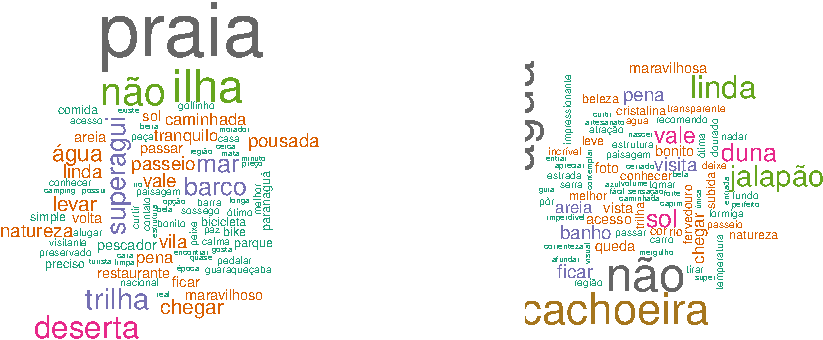
\includegraphics{bookdown-artigo_files/figure-latex/fig2-1} 

}

\caption{Wordcloud de unigramas}\label{fig:fig2}
\end{figure}

\begin{figure}[H]

{\centering 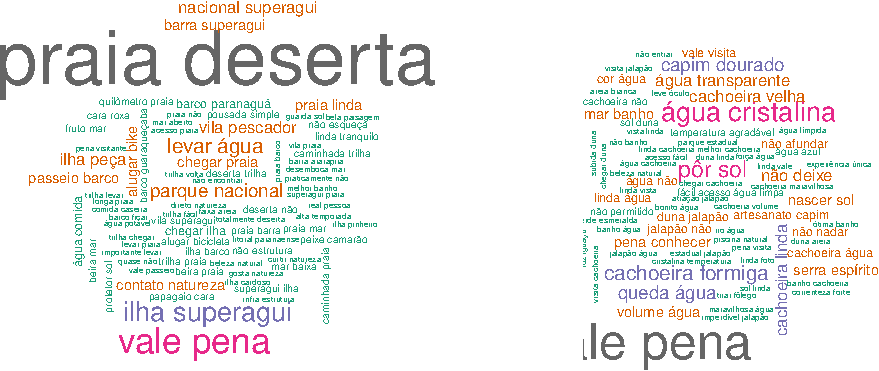
\includegraphics{bookdown-artigo_files/figure-latex/fig3-1} 

}

\caption{Wordcloud de bigramas}\label{fig:fig3}
\end{figure}

\hypertarget{frequencia-td-idf}{%
\subsection{Frequencia td-idf}\label{frequencia-td-idf}}

A ideia do \texttt{tf-idf} é encontrar as palavras importantes para o
conteúdo de cada documento diminuindo o peso das palavras comumente
usadas e aumentando o peso das palavras que não são muito usadas em uma
coleção ou \emph{corpus} de documentos, neste caso, o grupo de atrativos
turísticos. O cálculo do \texttt{tf-idf} tenta encontrar as palavras que
são importantes/comuns em um texto, mas não muito comuns.

A função \texttt{bind\_tf\_idf()} no pacote \emph{tidytext} recebe um
conjunto de dados de texto organizado como entrada com uma linha por
\emph{token} (termo), por documento. Uma coluna contém os termos, outra
coluna contém os atrativos e a última coluna contém as contagens, ou
quantas vezes cada atrativo contém cada termo. Normalmente, \texttt{idf}
e, portanto, \texttt{tf-idf} são zero para essas palavras extremamente
comuns. Estas são todas as palavras que aparecem em todos os dois
atrativos, então o termo \texttt{idf} (que será então o logaritmo
natural de 1 é zero. A frequência inversa do documento \texttt{tf-idf} é
muito baixa (próxima de zero) para palavras que ocorrem em muitos dos
documentos em uma coleção. É assim que essa abordagem diminui o peso das
palavras comuns. A frequência de documento inversa será um número maior
para palavras que ocorrem em menos documentos na coleção.

\begin{figure}[H]

{\centering 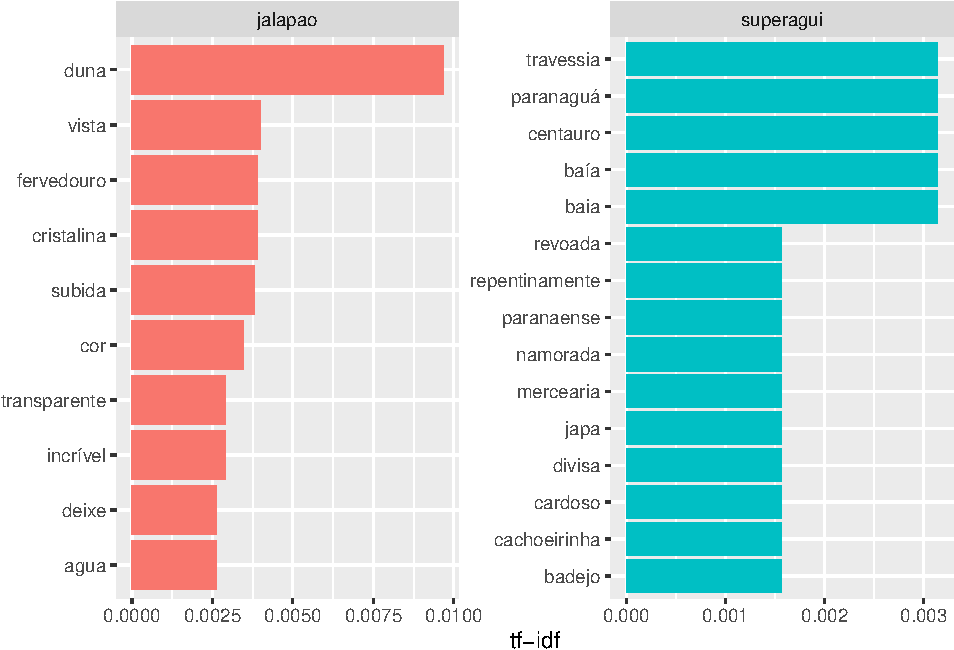
\includegraphics{bookdown-artigo_files/figure-latex/fig4-1} 

}

\caption{Frequência td-idf dos atrativos Jalapão e Superagui}\label{fig:fig4}
\end{figure}

A Figura \ref{fig:fig4} mostra a frequência \texttt{td-idf} entre os
atrativos turísticos utilizados como caso de estudo.

\begin{figure}[H]

{\centering 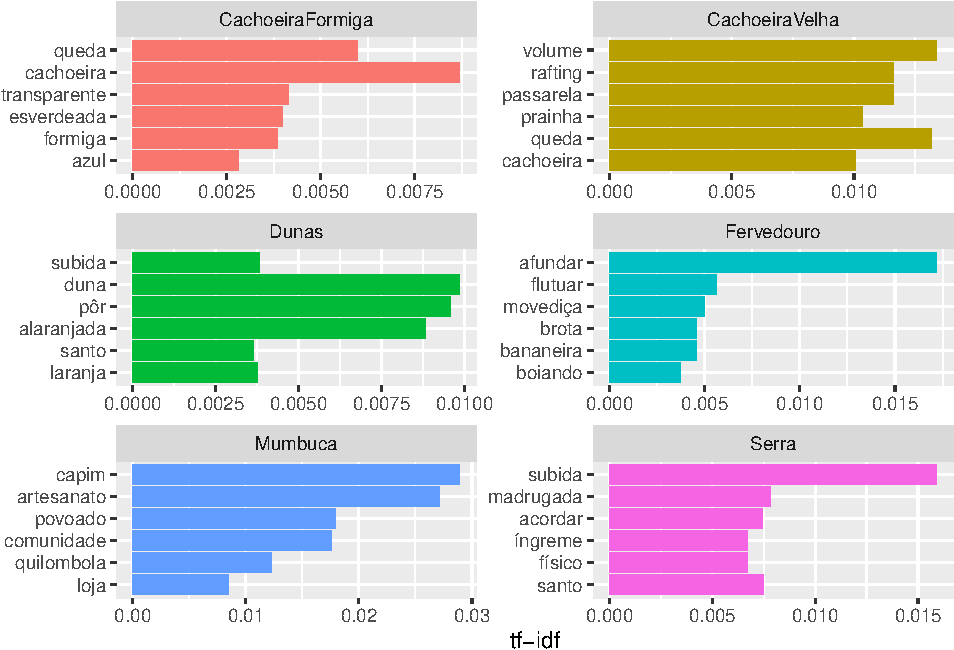
\includegraphics{bookdown-artigo_files/figure-latex/fig5-1} 

}

\caption{Frequência td-idf dos atrativos do Jalapão}\label{fig:fig5}
\end{figure}

A Figura \ref{fig:fig5}, mostra outro exemplo, agora dividindo os
atrativos existentes dentro do Jalapão.

\hypertarget{anuxe1lise-de-sentimentos}{%
\subsection{Análise de sentimentos}\label{anuxe1lise-de-sentimentos}}

A avaliação da experiência turística é um processo complexo, que envolve
a análise de diversos fatores, como o atendimento ao cliente, a
qualidade dos serviços oferecidos, o ambiente e a cultura local, entre
outros. A análise de sentimentos pode ser uma ferramenta útil para
avaliar a experiência turística, pois permite capturar e quantificar as
emoções expressas pelos turistas em relação a diferentes aspectos da
viagem. Com a análise de sentimentos, é possível identificar as emoções
positivas e negativas associadas a cada experiência turística, e
utilizar essas informações para melhorar a qualidade dos serviços
oferecidos (Figuras \ref{fig:fig8} e \ref{fig:fig9}).

\begin{figure}[H]

{\centering 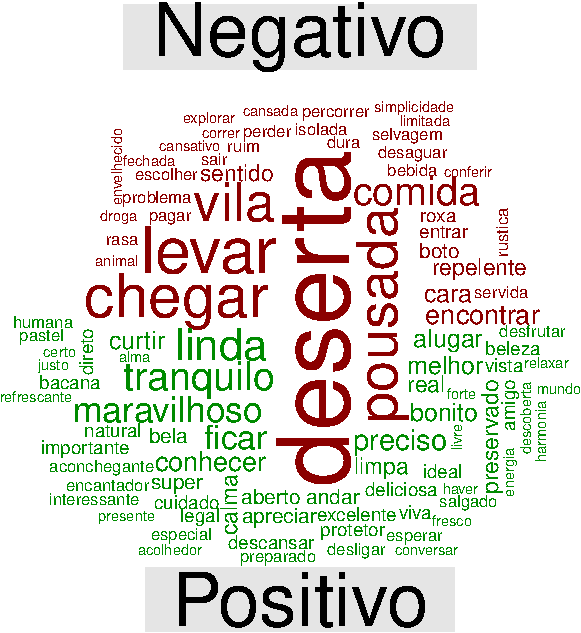
\includegraphics{bookdown-artigo_files/figure-latex/fig8-1} 

}

\caption{Análise de sentimentos de Superagui}\label{fig:fig8}
\end{figure}

\begin{figure}[H]

{\centering 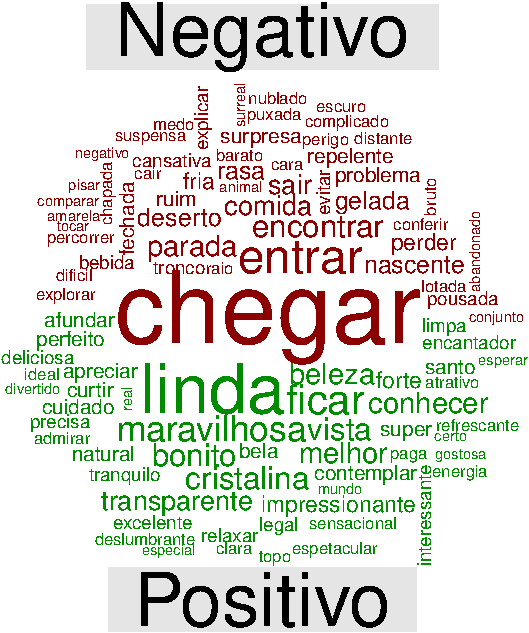
\includegraphics{bookdown-artigo_files/figure-latex/fig9-1} 

}

\caption{Análise de sentimentos do Jalapão}\label{fig:fig9}
\end{figure}

\hypertarget{clusterizauxe7uxe3o}{%
\subsection{Clusterização}\label{clusterizauxe7uxe3o}}

Em termos de clustering hierárquico, a esparsidade refere-se à presença
de grupos de dados com poucas observações. Esses grupos são assim
considerados porque têm poucos pontos de dados em relação aos outros
grupos. Ao realizar uma análise de cluster, é importante levar em
consideração a esparsidade e como ela pode afetar o resultado. Uma forma
de lidar com ela é aplicar técnicas de agrupamento aglomerativo que
considerem a distância entre grupos ponderando a densidade dos grupos.
Alguns métodos, como o método ``ward.D2'' no R, tentam minimizar a
variância total dos grupos e levando em consideração a esparsidade
(Figuras \ref{fig:fig10} e \ref{fig:fig11}).

No aplicativo \emph{shiny}, existe a opção de ajuste de esparsidade de
forma a ajudar na interpretação dos resultados da análise. O método
``ward.D2'' ainda não foi implementado no aplicativo, que, por enquanto,
está usando apenas a distância euclidiana.

\begin{figure}[H]

{\centering 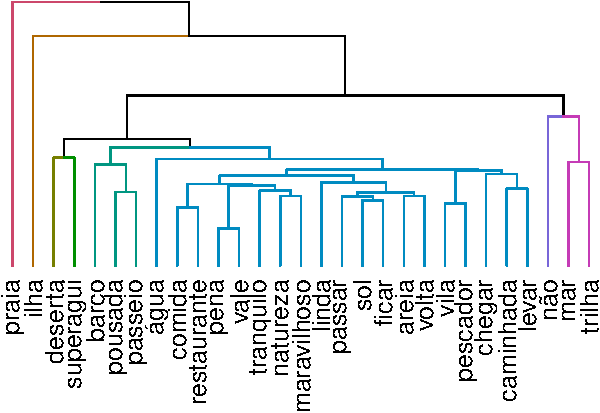
\includegraphics{bookdown-artigo_files/figure-latex/fig10-1} 

}

\caption{Dendrograma de Superagui}\label{fig:fig10}
\end{figure}

\begin{figure}[H]

{\centering 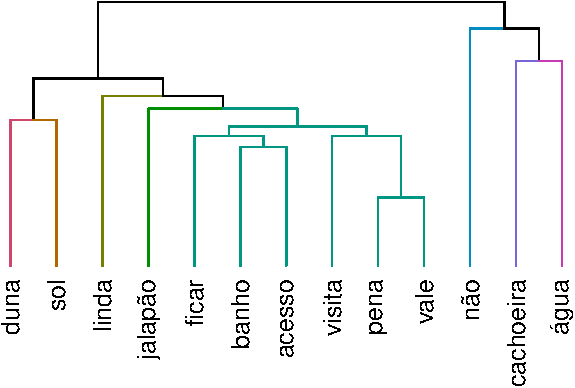
\includegraphics{bookdown-artigo_files/figure-latex/fig11-1} 

}

\caption{Dendrograma do Jalapão}\label{fig:fig11}
\end{figure}

\hypertarget{rede-de-palavras}{%
\subsection{Rede de Palavras}\label{rede-de-palavras}}

Foi realizada a distribuição de palavras sucessoras, ou redes de
palavras (Figura \ref{fig:fig6} e \ref{fig:fig7}), também conhecidas
como redes léxicas ou grafos de palavras, que são representações
gráficas que mostram as relações entre as palavras em um determinado
\emph{corpus} de texto. O resultado é a construção de conjuntos de
palavras que fornecem maior sentido que termos isolados. Cada palavra é
representada por um nó na rede, e as conexões entre elas são
representadas por arestas que indicam a frequência e a força das
relações entre as palavras. A utilidade das redes de palavras está na
capacidade de mostrar as associações semânticas entre as palavras em um
corpus, ajudando a identificar tópicos ou temas importantes,
palavras-chave e padrões linguísticos
(\protect\hyperlink{ref-Fay2018}{Fay 2018}).

\begin{figure}[H]

{\centering 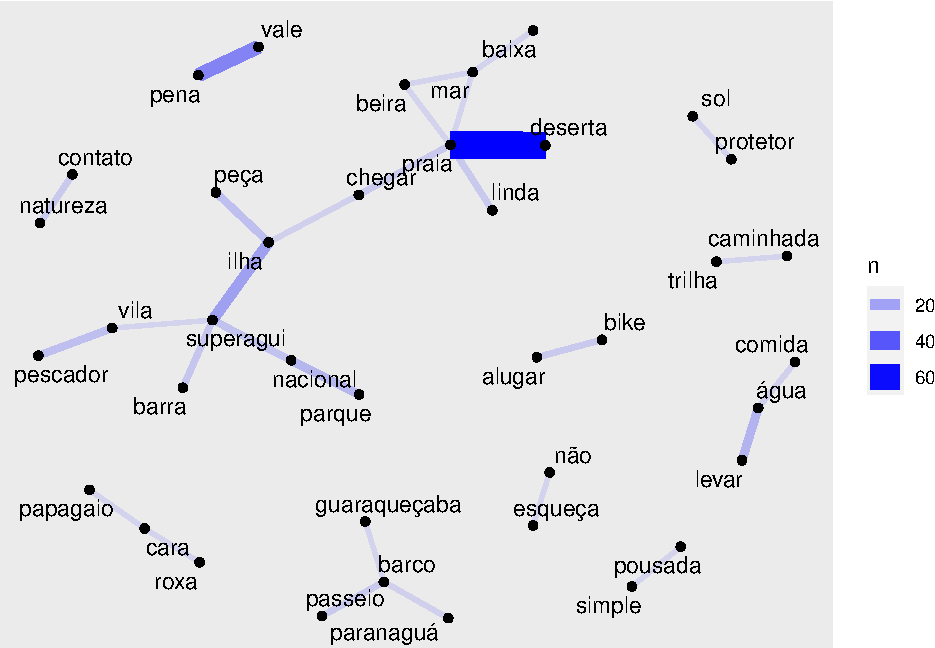
\includegraphics{bookdown-artigo_files/figure-latex/fig6-1} 

}

\caption{Redes de bigramas de Superagui}\label{fig:fig6}
\end{figure}

\begin{figure}[H]

{\centering 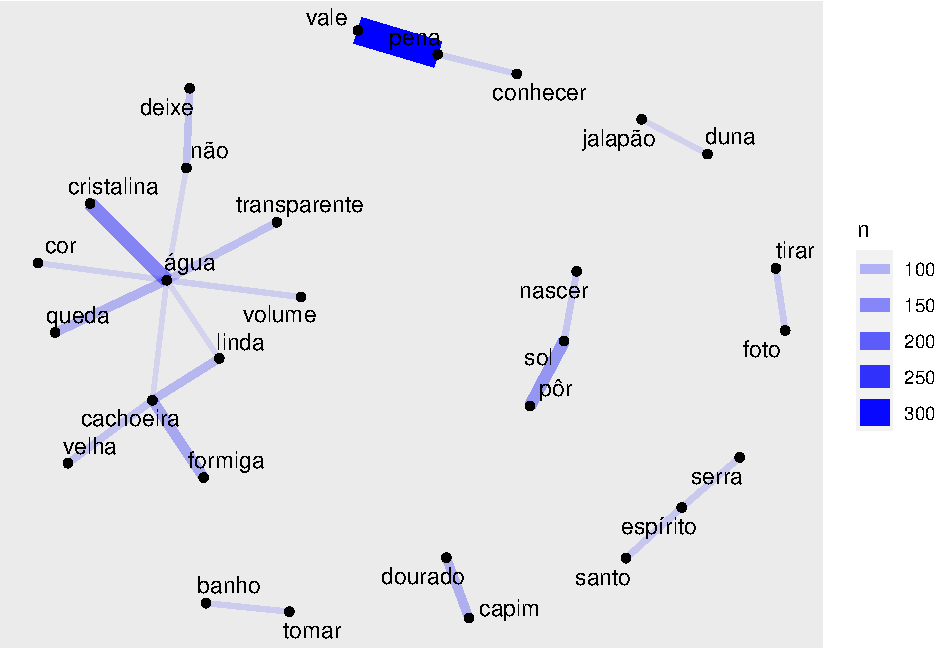
\includegraphics{bookdown-artigo_files/figure-latex/fig7-1} 

}

\caption{Redes de bigramas do Jalapão}\label{fig:fig7}
\end{figure}

\hypertarget{anuxe1lise-de-tuxf3picos}{%
\subsection{Análise de tópicos}\label{anuxe1lise-de-tuxf3picos}}

A LDA é um dos algoritmos mais comuns para modelagem de tópicos. Sem
mergulhar na matemática por trás do modelo, podemos entendê-lo como
sendo guiado por dois princípios. O primeiro é que cada documento é uma
mistura de tópicos. Imaginamos que cada documento pode conter palavras
de vários tópicos em proporções particulares. Por exemplo, em um modelo
de dois tópicos, poderíamos dizer ``Documento 1 é 90\% do tópico A e
10\% do tópico B, enquanto o Documento 2 é 30\% do tópico A e 70\% do
tópico B''. O segundo prinçipio é que cada tópico é uma mistura de
palavras, onde cada tópico possui palavras relacionadas a ele, porém, as
palavras podem ser compartilhadas entre os tópicos. A LDA é um método
matemático para estimar ambos ao mesmo tempo: encontrar a mistura de
palavras que está associada a cada tópico, ao mesmo tempo em que
determina a mistura de tópicos que descreve cada documento. A vantagem
da modelagem de tópicos em oposição aos métodos de ``agrupamento
rígido'' é que os tópicos usados em linguagem natural podem ter alguma
sobreposição em termos de palavras (\protect\hyperlink{ref-Fay2018}{Fay
2018}).

Nesse caso ilustrativo, utilizamos apenas um atrativo turístico para
analisar os tópicos, porém a análise pode ser feita com mais de um
atrativo ao mesmo tempo. Da mesma maneira que as outras análises, ela
pode ser feita a partir de diferentes n-gramas, mas deve-se considerar a
esparsidade com que longos n-gramas possuem.

\begin{figure}[H]

{\centering 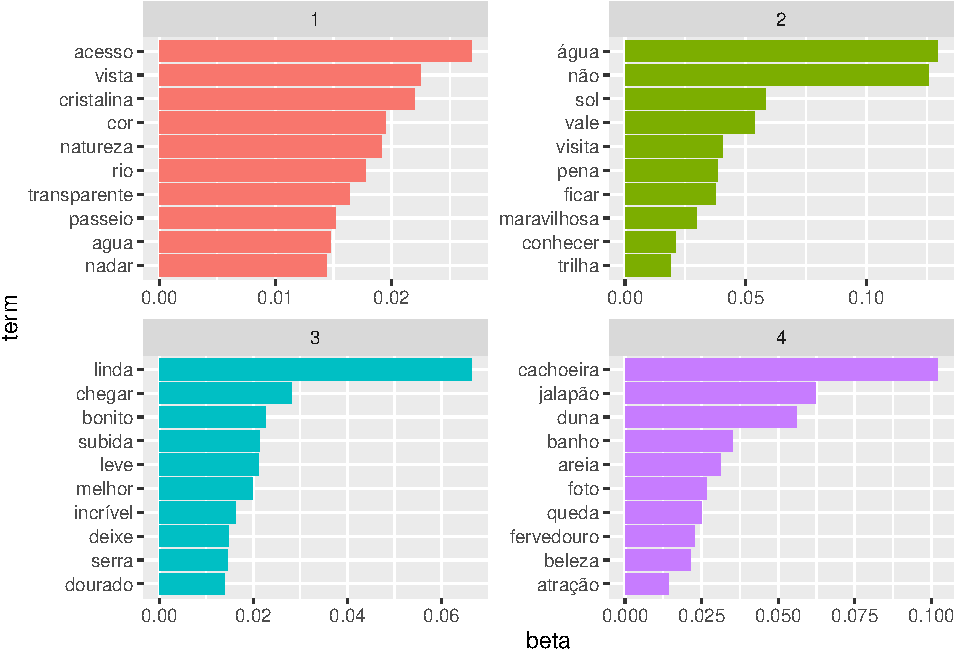
\includegraphics{bookdown-artigo_files/figure-latex/fig12-1} 

}

\caption{Análise de tópicos do Jalapão}\label{fig:fig12}
\end{figure}

A Figura \ref{fig:fig12} mostra uma análise de tópicos gerada para o
Jalapão. O pacote de \emph{tidytext} fornece um método para extrair as
probabilidades por tópico por palavra, chamado \(\beta\) (``beta''), do
modelo. Este transforma o modelo em um formato de um tópico por termo
por linha. Para cada combinação, ele calcula a probabilidade daquele
termo ser gerado daquele tópico. A função slice\_max() do dplyr pode ser
usada para encontrar os n termos mais comuns em cada tópico.

Como alternativa a primeira análise (Figura \ref{fig:fig13}), pode-se
considerar os termos que tiveram a maior diferença de \(\beta\) entre o
tópico 1 e o tópico 2. Isso pode ser estimado com base na razão
logarítmica dos dois (uma razão logarítmica é útil porque torna a
diferença simétrica: \(\beta2\) sendo duas vezes maior leva a uma razão
logarítmica de 1, enquanto \(\beta1\) sendo duas vezes maior resulta em
-1). Para restringi-lo a um conjunto de palavras especialmente
relevantes, pode-se filtrar por palavras relativamente comuns, como
aquelas que têm um \(\beta\) superior a 1/1000 em pelo menos um tópico.

\begin{figure}[H]

{\centering 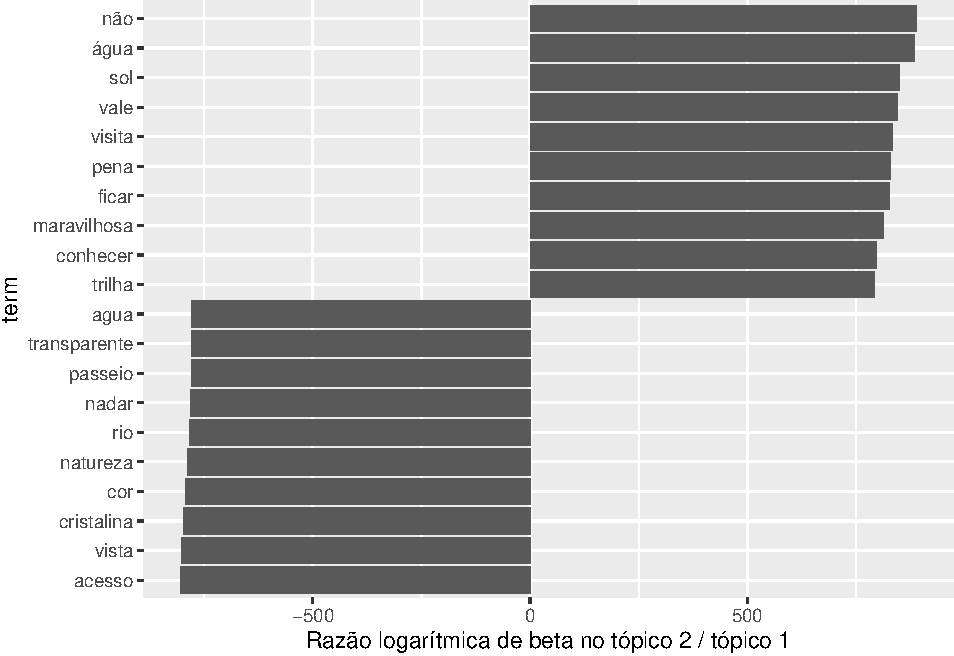
\includegraphics{bookdown-artigo_files/figure-latex/fig13-1} 

}

\caption{Análise de tópicos do Jalapão}\label{fig:fig13}
\end{figure}

\hypertarget{conclusuxe3o}{%
\section{Conclusão}\label{conclusuxe3o}}

Este artigo explorou as características e as potencialidades do pacote
\emph{Shiny} do software R para o desenvolvimento de um aplicativo
\emph{web} voltado à mineraçao de textos e análise de experiências
turíticas. Através de um conjunto de passos que asseguram a captura e
organização automática dos dados, pode-se realizar uma análise eficiente
dos textos de comentários de turistas. Além da utilização de diversas
funções estatísticas bastante conhecidas, foram desenvolvidas algumas
funções específicas para o processamento de textos, as quais ainda não
estavam disponíveis para o software R (\protect\hyperlink{ref-R-base}{R
Core Team 2023}). A proposta envolveu o desenvolvimento de um conjunto
de instrumentos para o processamento de dados textuais e visualização
destes na forma de tabelas, gráficos, dendrogramas, dentre outros. Isso
pode ajudar empresas de turismo e hospitalidade a melhorar a experiência
do usuário, identificando áreas de melhoria e desenvolvendo estratégias
para atender às expectativas dos clientes.

Sabe-se que existem outros \emph{softwares} que realizam este trabalho,
todavia, o analista fica restrito as funcionalidades inerentes ao
\emph{software}. Nesse sentido, a proposta neste trabalho é fornecer uma
ferramenta flexível e de baixo custo para o usuário, que permita a
supressão ou inclusão de funcionalidades conforme as suas necessidades.

A fim de testar o instrumento e validar os procedimentos, foram feitos
dois estudos de casos, para os quais foi seguido o procedimento
desenvolvido, possibilitando coletar os dados e organizá-los como
pretendido. Com os testes preliminares, ficou demonstrado que a
abordagem consegue capturar e organizar automaticamente os dados.

Algumas análises ainda estão em fase de implementação do app, como a
análise de frequência \emph{td-idf}, outros métodos de clusterização
para dados esparsos (como o ``ward.2'') e a análise de tópicos para um
conjunto de vários atrativos ao mesmo tempo, bem como a sua forma de
visualização invertida. Além disso, alguns ajustes ainda precisam ser
feitos, tanto na interface visual do usuário (front-end) como tamanho
dos plots, quanto no tempo de processamento e otimização do código.

A continuidade da pesquisa envolve a escolha do n-grama mais
representativo para a classificação manual destes por especialistas, de
modo a criar um conjunto robusto de dados de treinamento para posterior
aplicação de algoritmos de análise supervisionada, de forma a gerar
classificações automáticas para novos conjuntos de dados; bem como a
aplicação dessa metodologia juntamente com especialistas da área do
turismo, a fim de desenvolver e verificar possibilidades analíticas em
situações reais de tomada de decisão.

\hypertarget{referuxeancias}{%
\section*{Referências}\label{referuxeancias}}
\addcontentsline{toc}{section}{Referências}

\hypertarget{refs}{}
\begin{CSLReferences}{1}{0}
\leavevmode\vadjust pre{\hypertarget{ref-Alencar2019}{}}%
Alencar, Débora Gonçalves, Marina Lima dos Santos, Adriely Andrade e
Souza, and José Manoel Gonçalves Gândara. 2019. {``Produtos Turísticos
Para Demandantes de Experiências Da Dimensão Entretenimento de Pine
\&Amp; Gilmore: Novas Características e Tendências Para o Paraná.''}
\emph{Turismo Visão e Ação} 21 (June): 46.
\url{https://doi.org/10.14210/rtva.v21n2.p46-67}.

\leavevmode\vadjust pre{\hypertarget{ref-Andrukiu2015}{}}%
Andrukiu, A, and José M G Gândara. 2015. {``As Emoções No Destino:
Classificando Os Atrativos Turísticos de Antonina, Paraná (Brasil).''}
\emph{Revista Hospitalidade} XII.

\leavevmode\vadjust pre{\hypertarget{ref-Aroeira2016}{}}%
Aroeira, Tiago, Ana Carmem Dantas, and Marlusa De Sevilha Gosling. 2016.
{``Experiência Turística Memorável, Percepção Cognitiva, Reputação e
Lealdade Ao Destino: Um Modelo Empírico.''} \emph{Turismo - Visão e
Ação} 18. \url{https://doi.org/10.14210/rtva.v18n3.p584-610}.

\leavevmode\vadjust pre{\hypertarget{ref-Bakulina2008}{}}%
Bakulina, Marina P. 2008. {``Application of the Zipf Law to Text
Compression.''} \emph{Journal of Applied and Industrial Mathematics} 2.
\url{https://doi.org/10.1134/S1990478908040042}.

\leavevmode\vadjust pre{\hypertarget{ref-bardin2011}{}}%
Bardin, Laurence. 2011. \emph{Análise de Conteúdo}. Paperback; Edições
70.

\leavevmode\vadjust pre{\hypertarget{ref-beni2019}{}}%
Beni, M. C. 2019. \emph{An{á}lise Estrutural Do Turismo}. Editora Senac
S{ã}o Paulo. \url{https://books.google.com.br/books?id=f9GCDwAAQBAJ}.

\leavevmode\vadjust pre{\hypertarget{ref-Beni2004}{}}%
Beni, Mário Carlos. 2004. {``Turismo : Da Economia de Serviços à
Economia Da Experiência.''} \emph{Turismo Visão e Ação} 6.

\leavevmode\vadjust pre{\hypertarget{ref-Bezerra2014}{}}%
Bezerra, Cicero Aparecido, and André José Ribeiro Guimarães. 2014.
{``Mineração de Texto Aplicada Às Publicações Científicas Sobre Gestão
Do Conhecimento No Período de 2003 a 2012.''} \emph{Perspectivas Em
Ciência Da Informação} 19. \url{https://doi.org/10.1590/1981-5344/1834}.

\leavevmode\vadjust pre{\hypertarget{ref-Carosia2020}{}}%
Carosia, A. E. O., G. P. Coelho, and A. E. A. Silva. 2020. {``Analyzing
the Brazilian Financial Market Through Portuguese Sentiment Analysis in
Social Media.''} \emph{Applied Artificial Intelligence} 34.
\url{https://doi.org/10.1080/08839514.2019.1673037}.

\leavevmode\vadjust pre{\hypertarget{ref-Coelho2007}{}}%
Coelho, André, and Leticia Ribeiro. 2007. {``A Economia Da
Experiência.''} \emph{Observatório de Inovação Do Turismo} 2: 1--3.
\href{https://www.ebape.fgv.br/revistaoit}{www.ebape.fgv.br/revistaoit}.

\leavevmode\vadjust pre{\hypertarget{ref-Hott2023}{}}%
Corrêa, Stela Cristina Hott, and Marlusa De Sevilha Gosling. 2023. {``A
Experiência Turística Inteligente Na Perspectiva Do Viajante.''}
\emph{Turismo: Visão e Ação} 25.
\url{https://doi.org/10.14210/rtva.v25n1.p72-93}.

\leavevmode\vadjust pre{\hypertarget{ref-Duarte2012}{}}%
Duarte, Eduardo Santos. 2012. {``Sentiment Analysis on Twitter for the
Portuguese Language.''} \emph{Lncs}.

\leavevmode\vadjust pre{\hypertarget{ref-Fay2018}{}}%
Fay, Colin. 2018. {``Text Mining with r : A Tidy Approach.''}
\emph{Journal of Statistical Software} 83.
\url{https://doi.org/10.18637/jss.v083.b01}.

\leavevmode\vadjust pre{\hypertarget{ref-feinerer2014text}{}}%
Feinerer, Ingo, Kurt Hornik, et al. 2014. {``Text Mining Package.''}
\emph{R Reference Manual, R-Project.org}. \url{https://doi.org/1}.

\leavevmode\vadjust pre{\hypertarget{ref-vieira2015}{}}%
Freitas, Larissa A. De, and Renata Vieira. 2016. {``Exploring Resources
for Sentiment Analysis in Portuguese Language.''} In \emph{Proceedings -
2015 Brazilian Conference on Intelligent Systems, BRACIS 2015}.
\url{https://doi.org/10.1109/BRACIS.2015.52}.

\leavevmode\vadjust pre{\hypertarget{ref-galili2014dendextend}{}}%
Galili, Tal. 2014. {``Dendextend: Extending r's Dendrogram
Functionality.''} \emph{R Package Version 0.17} 5.
\url{https://doi.org/1}.

\leavevmode\vadjust pre{\hypertarget{ref-lexiconPT}{}}%
Gonzaga, Sillas. 2022. {``Lexicons for Portuguese Text Analysis.''}
\emph{The Journal of Open Source Software}, 5.
\url{https://cran.r-project.org/web/packages/lexiconPT/lexiconPT.pdf}.

\leavevmode\vadjust pre{\hypertarget{ref-Hocking2019}{}}%
Hocking, Toby Dylan. 2019. {``Comparing namedCapture with Other r
Packages for Regular Expressions.''} \emph{R Journal} 11.
\url{https://doi.org/10.32614/rj-2019-050}.

\leavevmode\vadjust pre{\hypertarget{ref-Horodyski2015}{}}%
Horodyski, Graziela Scalise, Diogo Lüders Fernandes, and José Manoel
Gonçalves Gândara. 2015. {``As Experiências Dos Turistas Em
Estabelecimentos Comerciais de Souvenirs No Destino Curitiba-Brasil.''}
\emph{Investigaciones Turísticas}.
\url{https://doi.org/10.14198/inturi2015.10.08}.

\leavevmode\vadjust pre{\hypertarget{ref-Hvitfeldt2021}{}}%
Hvitfeldt, Emil, and Julia Silge. 2021. \emph{Supervised Machine
Learning for Text Analysis in r}. \emph{Supervised Machine Learning for
Text Analysis in R}. \url{https://doi.org/10.1201/9781003093459}.

\leavevmode\vadjust pre{\hypertarget{ref-Johnson2020}{}}%
Johnson, Paul. 2020. {``R Markdown: The Definitive Guide.''} \emph{The
American Statistician} 74.
\url{https://doi.org/10.1080/00031305.2020.1745577}.

\leavevmode\vadjust pre{\hypertarget{ref-LoBuono2016}{}}%
LoBuono, Raquel, Marlusa De Sevilha Gosling, Carlos Alberto Gonçalves,
and Sandro Alves Medeiros. 2016. {``Relações Entre Dimensões Da
Experiência, Satisfação, Recomendação e Intenção de Retornar: A
Percepção de Participantes de Evento Cultural Resumo.''} \emph{PODIUM
Sport, Leisure and Tourism Review} 5.
\url{https://doi.org/10.5585/podium.v5i2.158}.

\leavevmode\vadjust pre{\hypertarget{ref-Lopes2022}{}}%
Lopes, Emerson, Larissa Freitas, Gabriel Gomes, Gerônimo Lemos, Luiz
Hammes, and Ulisses Corrêa. 2022. {``Exploring BERT for Aspect-Based
Sentiment Analysis in Portuguese Language.''} In \emph{Proceedings of
the International Florida Artificial Intelligence Research Society
Conference, FLAIRS}. Vol. 35.
\url{https://doi.org/10.32473/flairs.v35i.130601}.

\leavevmode\vadjust pre{\hypertarget{ref-munzert2014automated}{}}%
Munzert, Simon, Christian Rubba, Peter Meißner, and Dominic Nyhuis.
2014. \emph{Automated Data Collection with {R}: A Practical Guide to Web
Scraping and Text Mining}. John Wiley \& Sons.

\leavevmode\vadjust pre{\hypertarget{ref-nunes2021}{}}%
Oliveira, Douglas Nunes de, and Luiz Henrique de Campos Merschmann.
2021. {``Joint Evaluation of Preprocessing Tasks with Classifiers for
Sentiment Analysis in Brazilian Portuguese Language.''} \emph{Multimedia
Tools and Applications} 80.
\url{https://doi.org/10.1007/s11042-020-10323-8}.

\leavevmode\vadjust pre{\hypertarget{ref-Pereira2021}{}}%
Pereira, Denilson Alves. 2021. {``A Survey of Sentiment Analysis in the
Portuguese Language.''} \emph{Artificial Intelligence Review} 54.
\url{https://doi.org/10.1007/s10462-020-09870-1}.

\leavevmode\vadjust pre{\hypertarget{ref-pine1999}{}}%
Pine, Joseph B, and James H Gilmore. 1998. {``Welcome to the Experience
Economy.''} \emph{Harvard Business Review}, 97--105.

\leavevmode\vadjust pre{\hypertarget{ref-R-base}{}}%
R Core Team. 2023. \emph{R: A Language and Environment for Statistical
Computing}. Vienna, Austria: R Foundation for Statistical Computing.
\url{https://www.R-project.org/}.

\leavevmode\vadjust pre{\hypertarget{ref-R-broom}{}}%
Robinson, David. 2017. \emph{{broom}: Convert Statistical Analysis
Objects into Tidy Data Frames}.
\url{https://CRAN.R-project.org/package=broom}.

\leavevmode\vadjust pre{\hypertarget{ref-RStudio2017}{}}%
RStudio. 2017. {``Basic Regular Expressions in r.''} \emph{Cheat Sheet}.

\leavevmode\vadjust pre{\hypertarget{ref-RStudio2018}{}}%
---------. 2018. {``Shiny - RStudio.''} \emph{RStudio}.

\leavevmode\vadjust pre{\hypertarget{ref-Sarica2021}{}}%
Sarica, Serhad, and Jianxi Luo. 2021. {``Stopwords in Technical Language
Processing.''} \emph{PLoS ONE} 16.
\url{https://doi.org/10.1371/journal.pone.0254937}.

\leavevmode\vadjust pre{\hypertarget{ref-Sharma2020}{}}%
Sharma, Aman, and Rishi Rana. 2020. {``Analysis and Visualization of
Twitter Data Using r.''} In \emph{PDGC 2020 - 2020 6th International
Conference on Parallel, Distributed and Grid Computing}.
\url{https://doi.org/10.1109/PDGC50313.2020.9315740}.

\leavevmode\vadjust pre{\hypertarget{ref-Silge2017}{}}%
Silge, Julia, and David Robinson. 2017. \emph{Welcome to Text Mining
with r}. \emph{Development}.

\leavevmode\vadjust pre{\hypertarget{ref-Tan1999}{}}%
Tan, Ah-Hwee. 1999. {``Text Mining: The State of the Art and the
Challenges.''} \emph{Proceedings of the PAKDD 1999 Workshop on Knowledge
Disocovery from Advanced Databases} 8.
\url{https://doi.org/10.1.1.38.7672}.

\leavevmode\vadjust pre{\hypertarget{ref-medeiros2021}{}}%
Tereza Medeiros, José Mendes, Mariana Sousa. 2021. {``A IMPORTÂNCIA DAS
TECNOLOGIAS DE INFORMAÇÃO e COMUNICAÇÃO NO TURISMO SÉNIOR: UMA REVISÃO
SISTEMÁTICA.''} \emph{Turismo - Visão e Ação} 23.
\url{https://doi.org/10.14210/rtva.v23n3.p579-594}.

\leavevmode\vadjust pre{\hypertarget{ref-Tung2011}{}}%
Tung, Vincent Wing Sun, and J. R.Brent Ritchie. 2011. {``Exploring the
Essence of Memorable Tourism Experiences.''} \emph{Annals of Tourism
Research} 38. \url{https://doi.org/10.1016/j.annals.2011.03.009}.

\leavevmode\vadjust pre{\hypertarget{ref-R-ggplot2}{}}%
Wickham, Hadley. 2009. \emph{{ggplot2}: Elegant Graphics for Data
Analysis}. Springer-Verlag New York. \url{http://ggplot2.org}.

\leavevmode\vadjust pre{\hypertarget{ref-R-tidyr}{}}%
---------. 2016. \emph{{tidyr}: Easily Tidy Data with `Spread()` and
`Gather()` Functions}. \url{https://CRAN.R-project.org/package=tidyr}.

\leavevmode\vadjust pre{\hypertarget{ref-Wickham2019}{}}%
---------. 2019. {``Rvest Package \textbar{} r Documentation.''}
\emph{RDocumentation}.

\leavevmode\vadjust pre{\hypertarget{ref-R-dplyr}{}}%
Wickham, Hadley, and Romain Francois. 2016. \emph{{dplyr}: A Grammar of
Data Manipulation}. \url{https://CRAN.R-project.org/package=dplyr}.

\leavevmode\vadjust pre{\hypertarget{ref-Xie2016}{}}%
Xie, Yihui. 2016. \emph{Bookdown: Authoring Books and Technical
Documents with r Markdown}. \emph{Bookdown: Authoring Books and
Technical Documents with R Markdown}.
\url{https://doi.org/10.1201/9781315204963}.

\leavevmode\vadjust pre{\hypertarget{ref-Yadav2018}{}}%
Yadav, Virendra, Srushti Chahande, and Ankita Wandre. 2018. {``Review on
Twitter Data Analysis Using r Language.''} \emph{IJARCCE} 7.
\url{https://doi.org/10.17148/ijarcce.2018.71014}.

\leavevmode\vadjust pre{\hypertarget{ref-DT}{}}%
Yihui Xie, Xianying Tan, Joe Cheng. 2018. {``A Wrapper of the JavaScript
Library DataTables.''} \emph{The Journal of Open Source Software}, 5.
\url{https://rstudio.github.io/DT}.

\end{CSLReferences}


\end{document}
